\documentclass{ieeeaccess}
\usepackage{cite}
\usepackage{amsmath,amssymb,amsfonts}
\usepackage{graphicx}
\usepackage{textcomp}
\usepackage{url}

\newcommand{\DatasetCount}{10}
\newcommand{\SeedCount}{5}
\newcommand{\ModelCount}{5}
\newcommand{\SearchConfigsPerModel}{12}
\newcommand{\TotalRuns}{250}
\newcommand{\TotalModelFits}{3250}
\newcommand{\HardwareCPU}{Apple M3 Pro}
\newcommand{\HardwareRAM}{18 GB}
\newcommand{\BestMacroFOneModel}{Extra Trees}
\newcommand{\BestMacroFOneValue}{0.873}
\newcommand{\MLPMacroFOneValue}{0.852}
\newcommand{\ExtraTreesMacroGainVsMLP}{0.021}
\newcommand{\HGBMacroGainVsMLP}{0.017}
\newcommand{\RandomForestWinsVsMLP}{9}
\newcommand{\ExtraTreesWinsVsMLP}{8}
\newcommand{\HGBWinsVsMLP}{10}
\newcommand{\FriedmanPValue}{0.002}
\newcommand{\MLPMeanRank}{4.2}
\newcommand{\BestMeanRank}{2.1}
\newcommand{\MLPStability}{0.018}
\newcommand{\LogisticFitTime}{0.016}
\newcommand{\ExtraTreesFitTime}{0.176}
\newcommand{\MLPFitTime}{0.546}


\def\BibTeX{{\rm B\kern-.05em{\sc i\kern-.025em b}\kern-.08em
    T\kern-.1667em\lower.7ex\hbox{E}\kern-.125emX}}

\begin{document}

\history{Draft prepared on April 9, 2026.}
\doi{10.1109/ACCESS.2026.0000000}

\title{On a Laptop, Tree Ensembles Still Win: A Negative Result for Small Neural Baselines on Numerical Tabular Classification}

\author{\uppercase{Author Name}\authorrefmark{1}}

\address[1]{Author affiliation and contact information to be inserted before submission.}
\tfootnote{Code, experiment scripts, generated tables, and figures are included in the accompanying repository.}

\markboth
{Author Name: Tree Ensembles Still Win on a Laptop}
{Author Name: Tree Ensembles Still Win on a Laptop}

\corresp{Corresponding author: to be inserted before submission.}

\begin{abstract}
Neural models are frequently proposed as drop-in replacements for classical machine learning on tabular data, but many practitioners work under much smaller hyperparameter and runtime budgets than contemporary benchmark papers assume. This paper reports a negative result for that pragmatic setting. We evaluate Logistic Regression, Random Forest, Extra Trees, HistGradientBoosting, and a width-limited multilayer perceptron (MLP) on \DatasetCount{} public OpenML numerical tabular classification datasets spanning 768 to 19{,}020 samples, 4 to 57 features, and both binary and multiclass tasks. Each model receives the same \SearchConfigsPerModel{}-configuration validation budget on each of \SeedCount{} random seeds, producing \TotalModelFits{} total fits on an \HardwareCPU{} laptop with \HardwareRAM{} of unified memory. We report accuracy, macro-F1, Brier score, expected calibration error (ECE), search time, fit time, and seed stability. Extra Trees attains the best mean macro-F1 (\BestMacroFOneValue{}), followed closely by Random Forest and HistGradientBoosting, while the MLP ranks last overall among the non-linear baselines (\MLPMacroFOneValue{}; mean rank \MLPMeanRank{}). HistGradientBoosting beats the MLP on all ten datasets, Random Forest on \RandomForestWinsVsMLP{}, and Extra Trees on \ExtraTreesWinsVsMLP{}; the Friedman test over datasets is significant ($p=\FriedmanPValue$). The MLP also exhibits the highest seed-to-seed variability in both macro-F1 and calibration. These results do not rule out stronger neural architectures, but they do show that a modest MLP is not the pragmatic default for small-to-medium numerical tabular workloads under laptop-scale tuning budgets.
\end{abstract}

\begin{keywords}
benchmarking, calibration, classical machine learning, negative results, tabular classification.
\end{keywords}

\titlepgskip=-15pt
\maketitle

\section{Introduction}
\PARstart{T}{abular} classification remains one of the most common machine learning workloads in practice, yet model selection advice is often pulled from literature that assumes generous compute budgets and extensive hyperparameter search. For many applied settings, especially exploratory work conducted on a single laptop, the practical question is narrower: when the search budget is small and the datasets are modest, is a neural baseline actually the best default choice?

Recent benchmark studies have already challenged strong claims about deep learning on tabular data. Gorishniy \emph{et al.}\ cite{gorishniy2021} showed that carefully regularized MLP-style baselines are competitive with specialized tabular architectures, and Grinsztajn \emph{et al.}\ cite{grinsztajn2022} reported that tree-based models still outperform deep learning on many typical tabular datasets even after substantial tuning. Those papers are important, but their experimental scope and compute budgets are broader than what many small projects can afford in a single day on commodity hardware.

This paper narrows the question to a laptop-scale regime and asks whether a modest multilayer perceptron is a sensible default baseline for \emph{numerical} tabular classification when each model gets the same small validation budget. The answer, on the benchmark studied here, is no. Across \DatasetCount{} public datasets and \TotalRuns{} evaluated runs, the tree ensembles consistently outperform the MLP in macro-F1, usually improve calibration, and produce more stable results across random seeds. The goal is not to argue that neural models are categorically ineffective on tabular data, but to show that under tight budgets a simple MLP remains a weak practical default compared with tuned classical ensembles.

The contributions of this work are threefold:
\begin{itemize}
\item A reproducible laptop-scale benchmark covering \DatasetCount{} public numerical tabular classification datasets, five standard model families, and \TotalModelFits{} total fits under a fixed per-model validation budget.
\item A multi-metric comparison that includes macro-F1, accuracy, Brier score, ECE, search time, fit time, and seed stability rather than only point accuracy.
\item A negative empirical result: the MLP ranks last overall, while tree ensembles dominate aggregate performance and stability under the chosen compute budget.
\end{itemize}

\section{Related Work}
Large comparative studies long predate the current wave of tabular deep learning. Caruana and Niculescu-Mizil compared diverse supervised learning methods over multiple benchmark tasks and highlighted the importance of broad experimental evaluation. More recently, open benchmarking infrastructures such as OpenML have made it easier to package datasets, code, and exact evaluation settings for replication and extension \cite{vanschoren2014}.

Tree-based ensembles remain strong baselines for tabular data. Random Forests \cite{breiman2001} and Extremely Randomized Trees \cite{geurts2006} are widely used because they train quickly, tolerate heterogeneous feature scales, and often perform well with limited tuning. Gradient boosting methods, including the greedy function approximation formulation introduced by Friedman \cite{friedman2001}, are also standard high-performance choices for tabular prediction.

For neural models, two observations from the recent literature are especially relevant here. First, strong regularized MLP baselines are harder to beat than some papers suggest \cite{gorishniy2021}. Second, even after careful random search, tree-based models often remain superior on medium-scale tabular problems \cite{grinsztajn2022}. The present study aligns with that line of evidence, but focuses on a smaller and more explicitly budgeted setting: a width-limited MLP against classical baselines, all tuned under the same modest search budget on a single laptop.

Because negative results in benchmarking are only convincing when they are evaluated carefully, the statistical comparison follows Dem\v{s}ar's recommendations for multiple classifiers over multiple datasets \cite{demsar2006}. Calibration is reported with Brier score \cite{brier1950} and expected calibration error, following the modern calibration framing of Guo \emph{et al.}\ \cite{guo2017}.

\section{Experimental Design}
\subsection{Research Question}
The study tests the following hypothesis: under a laptop-scale hyperparameter budget on small-to-medium numerical tabular classification problems, carefully tuned classical models outperform a modest MLP not only in predictive performance but also in calibration and seed stability.

\subsection{Datasets}
The benchmark uses \DatasetCount{} public classification datasets loaded from OpenML \cite{vanschoren2014}. To keep preprocessing simple and isolate model behavior from categorical encoding choices, only numerical tabular datasets were included. Table~\ref{tab:datasets} summarizes the benchmark.

\begin{table}[!t]
\caption{Benchmark datasets. Minority share is the fraction of examples in the least frequent class.}
\label{tab:datasets}
\centering
\scriptsize
\resizebox{\columnwidth}{!}{\begin{tabular}{lrrrrrr}
\hline
Dataset & Task ID & Data ID & Samples & Features & Classes & Minority share \\
\hline
kc2 & 3913 & 1063 & 522 & 21 & 2 & 0.205 \\
climate-model-simulation-crashes & 146819 & 40994 & 540 & 18 & 2 & 0.085 \\
wdbc & 9946 & 1510 & 569 & 30 & 2 & 0.373 \\
balance-scale & 11 & 11 & 625 & 4 & 3 & 0.078 \\
blood-transfusion-service-center & 10101 & 1464 & 748 & 4 & 2 & 0.238 \\
diabetes & 37 & 37 & 768 & 8 & 2 & 0.349 \\
vehicle & 53 & 54 & 846 & 18 & 4 & 0.235 \\
qsar-biodeg & 9957 & 1494 & 1055 & 41 & 2 & 0.337 \\
pc1 & 3918 & 1068 & 1109 & 21 & 2 & 0.069 \\
banknote-authentication & 10093 & 1462 & 1372 & 4 & 2 & 0.445 \\
pc4 & 3902 & 1049 & 1458 & 37 & 2 & 0.122 \\
pc3 & 3903 & 1050 & 1563 & 37 & 2 & 0.102 \\
steel-plates-fault & 146817 & 40982 & 1941 & 27 & 7 & 0.028 \\
mfeat-morphological & 18 & 18 & 2000 & 6 & 10 & 0.100 \\
mfeat-zernike & 22 & 22 & 2000 & 47 & 10 & 0.100 \\
kc1 & 3917 & 1067 & 2109 & 21 & 2 & 0.155 \\
segment & 146822 & 40984 & 2310 & 16 & 7 & 0.143 \\
spambase & 43 & 44 & 4601 & 57 & 2 & 0.394 \\
wilt & 146820 & 40983 & 4839 & 5 & 2 & 0.054 \\
phoneme & 9952 & 1489 & 5404 & 5 & 2 & 0.293 \\
wall-robot-navigation & 9960 & 1497 & 5456 & 24 & 4 & 0.060 \\
first-order-theorem-proving & 9985 & 1475 & 6118 & 51 & 6 & 0.079 \\
satimage & 2074 & 182 & 6430 & 36 & 6 & 0.097 \\
GesturePhaseSegmentationProcessed & 14969 & 4538 & 9873 & 32 & 5 & 0.101 \\
pendigits & 32 & 32 & 10992 & 16 & 10 & 0.096 \\
\hline
\end{tabular}
}
\end{table}

\subsection{Models and Search Budget}
Five model families were evaluated:
\begin{enumerate}
\item Logistic Regression with standardized inputs.
\item Random Forest.
\item Extra Trees.
\item HistGradientBoosting.
\item A width-limited MLP with ReLU activations, Adam optimization, and early stopping.
\end{enumerate}

Every dataset-model-seed combination received the same validation budget: \SearchConfigsPerModel{} sampled hyperparameter configurations, selected from a predefined model-specific search space. The budget was intentionally small, reflecting the type of search a practitioner can reasonably finish on a laptop in under a day. This produces \TotalRuns{} final test evaluations and \TotalModelFits{} total fits when validation-search fits are counted.

\subsection{Protocol}
For each dataset and random seed, the data were split into 60\% train, 20\% validation, and 20\% test partitions using stratified sampling. Hyperparameters were selected by validation macro-F1. The best configuration was then retrained on the union of the training and validation partitions and evaluated on the held-out test partition.

Numerical preprocessing used median imputation for all models. Logistic Regression and the MLP additionally used standardization. The primary ranking metric was macro-F1 because several datasets are imbalanced or multiclass. Accuracy, Brier score, ECE, search time, fit time, and inference time were also recorded. Aggregate model comparisons over datasets were assessed with the Friedman test \cite{demsar2006}.

\subsection{Hardware}
All experiments ran on a single \HardwareCPU{} laptop with \HardwareRAM{} of unified memory running macOS 26.3.1. Summing wall-clock validation search and final training times across all runs yields about 23.7 minutes of total compute for the benchmark.

\section{Results}
\subsection{Aggregate Performance}
Table~\ref{tab:overall} reports the aggregate results. Extra Trees achieves the best mean macro-F1 (\BestMacroFOneValue{}), while Random Forest achieves the best mean rank (\BestMeanRank{}). HistGradientBoosting trails closely in macro-F1 and produces the best average calibration (ECE 0.032). The MLP reaches only \MLPMacroFOneValue{} mean macro-F1 and finishes last by average rank.

\begin{table}[!t]
\caption{Aggregate benchmark results across all datasets and seeds. Lower is better for rank, Brier, ECE, and time.}
\label{tab:overall}
\centering
\scriptsize
\resizebox{\columnwidth}{!}{\begin{tabular}{lrrrrrrr}
\hline
Model & Rank & Macro-F1 & Acc. & Brier & ECE & Search (s) & Fit (s) \\
\hline
Extra Trees & 2.3 & \textbf{0.873} & 0.902 & 0.138 & 0.047 & 2.48 & 0.176 \\
\textbf{Random Forest} & \textbf{2.1} & 0.872 & 0.902 & 0.140 & 0.046 & 4.04 & 0.333 \\
HistGradientBoosting & 2.4 & 0.869 & 0.900 & 0.144 & \textbf{0.032} & 15.12 & 1.313 \\
MLP & 4.2 & 0.852 & 0.890 & 0.165 & 0.049 & 4.22 & 0.546 \\
Logistic Regression & 4.0 & 0.835 & 0.857 & 0.201 & 0.043 & \textbf{0.16} & \textbf{0.016} \\
\hline
\end{tabular}
}
\end{table}

The negative-result signal is not marginal. Relative to the MLP, Extra Trees improves mean macro-F1 by \ExtraTreesMacroGainVsMLP{}, and HistGradientBoosting improves it by \HGBMacroGainVsMLP{}. The Friedman test across the five models is significant ($p=\FriedmanPValue$), indicating that the ranking differences are unlikely to be explained by random variation alone.

\subsection{Per-Dataset Comparison Against the MLP}
The MLP does not win the benchmark on any dataset. HistGradientBoosting outperforms the MLP on all \DatasetCount{} datasets, Random Forest on \RandomForestWinsVsMLP{}, and Extra Trees on \ExtraTreesWinsVsMLP{}. The only dataset won by a linear model is \textit{vehicle}, where Logistic Regression achieves the strongest macro-F1, indicating that the benchmark is not simply rewarding non-linearity by construction.

\begin{figure}[!t]
\centering
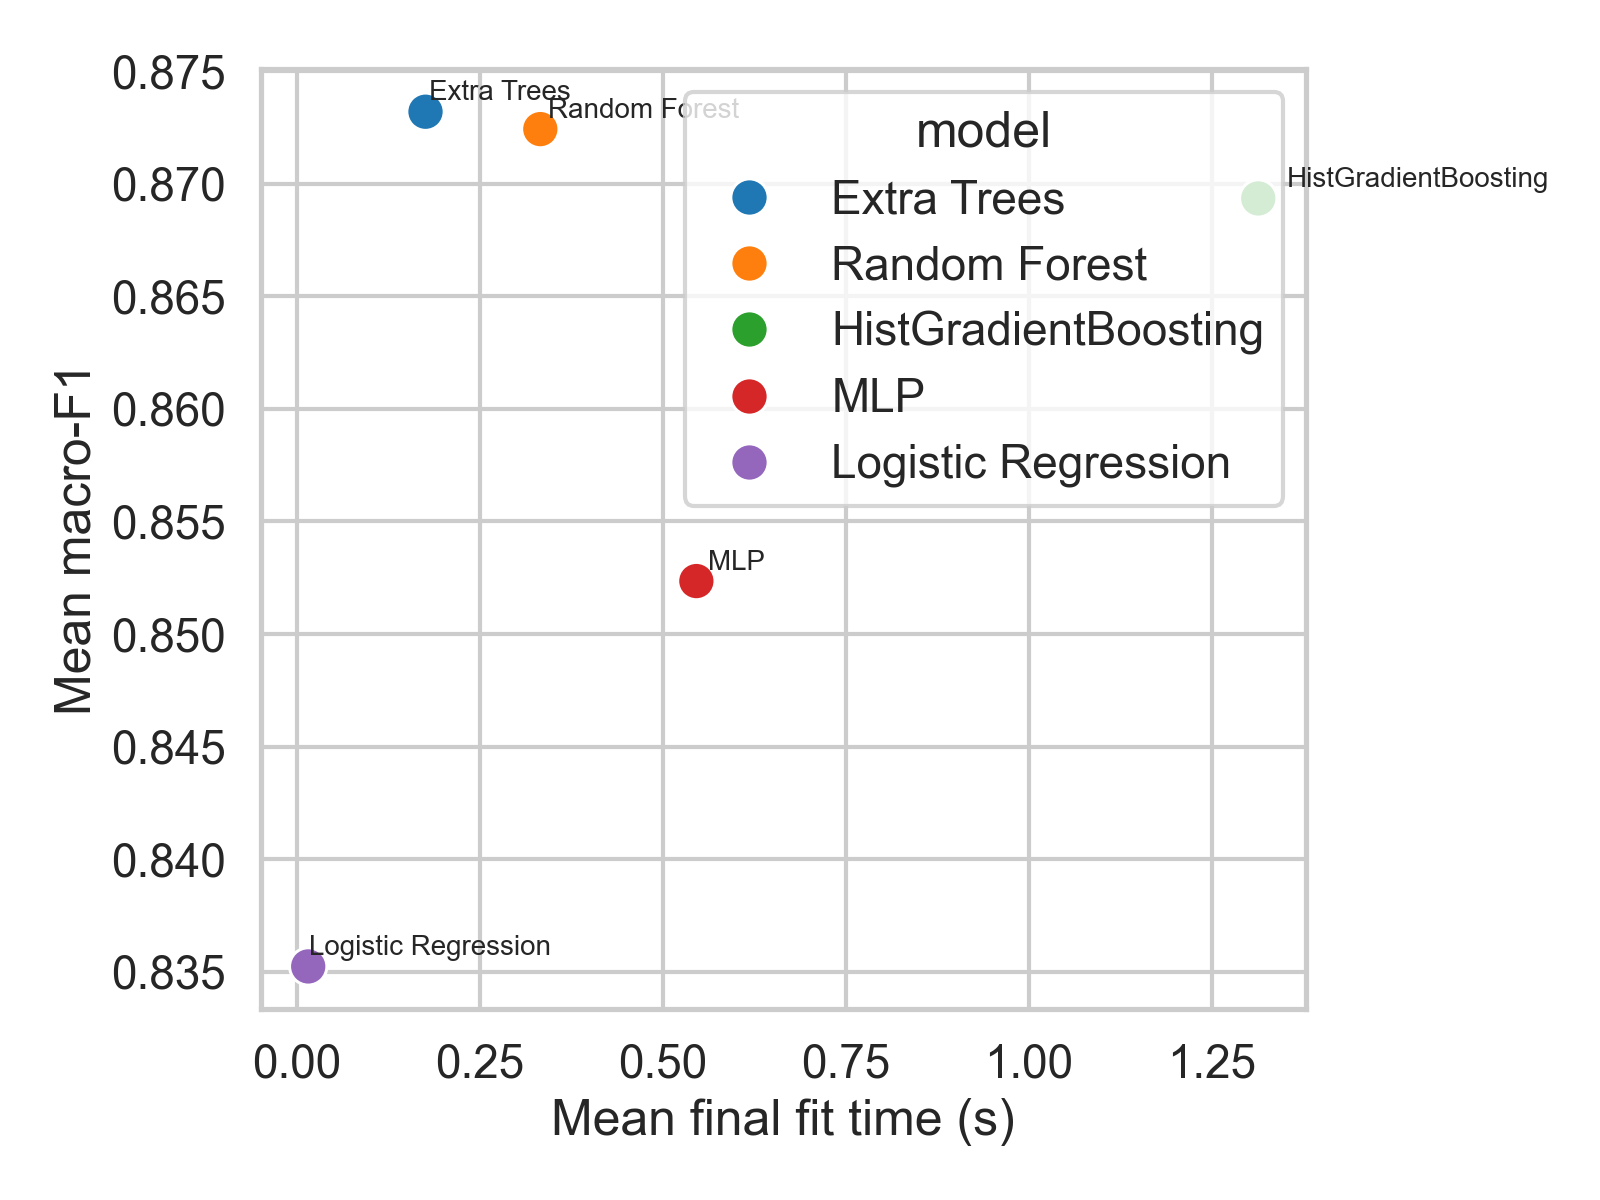
\includegraphics[width=\columnwidth]{../results/figures/macro_f1_vs_fit_time.png}
\caption{Aggregate macro-F1 versus final fit time. Extra Trees and Random Forest occupy the strongest part of the accuracy-time frontier, while the MLP is slower than these tree ensembles and less accurate.}
\label{fig:tradeoff}
\end{figure}

Figure~\ref{fig:tradeoff} summarizes the performance-time trade-off. Logistic Regression is the fastest model to search and fit, but it gives up too much predictive performance on most datasets. The more important practical observation is that the MLP is not competitive on the frontier either: it is substantially slower to fit than Extra Trees (\MLPFitTime{}~s versus \ExtraTreesFitTime{}~s on average) while still delivering lower macro-F1.

\subsection{Calibration and Stability}
Calibration and stability reinforce the same conclusion. HistGradientBoosting attains the best mean ECE, and the MLP has the worst average calibration variance across seeds. Table~\ref{tab:stability} shows that the MLP also has the largest mean seed-to-seed macro-F1 standard deviation (\MLPStability{}), while the classical baselines remain more stable.

\begin{table}[!t]
\caption{Average seed-to-seed variability aggregated over datasets. Lower is better.}
\label{tab:stability}
\centering
\scriptsize
\resizebox{\columnwidth}{!}{\begin{tabular}{lrrrr}
\hline
Model & Macro-F1 std & Acc. std & Brier std & ECE std \\
\hline
Logistic Regression & 0.012 & 0.015 & 0.017 & 0.011 \\
Random Forest & 0.013 & 0.009 & 0.010 & 0.009 \\
Extra Trees & 0.014 & 0.010 & 0.011 & 0.009 \\
HistGradientBoosting & 0.015 & 0.013 & 0.015 & 0.009 \\
MLP & 0.018 & 0.015 & 0.038 & 0.033 \\
\hline
\end{tabular}
}
\end{table}

This matters because in small-data regimes practitioners often run a model only a handful of times. A model family that is sensitive to initialization and split choice imposes additional hidden cost even when its average score looks acceptable. In this benchmark, the MLP is weaker both in mean performance and in repeatability.

\section{Discussion}
The results support a restrained but useful conclusion: on small-to-medium numerical tabular classification tasks, a modest MLP is not the pragmatic default under a fixed laptop-scale tuning budget. That conclusion is narrower than a universal claim about neural networks on tabular data, but it is also closer to a realistic day-to-day decision boundary for practitioners.

Three details are worth emphasizing. First, the tree ensembles do not win by an artifact of poor calibration reporting; they remain competitive or better even when Brier score and ECE are included. Second, the MLP is not simply undercut by a linear baseline, because the strongest competitors are usually non-linear ensembles rather than Logistic Regression. Third, the compute story matters: the MLP does not recover its weaker macro-F1 with a runtime advantage over the best-performing tree ensemble.

These findings are directionally consistent with the broader tabular deep learning literature \cite{gorishniy2021,grinsztajn2022}, but they also sharpen the practitioner-facing message. When the search budget is constrained to roughly two dozen minutes of total experiment time on a laptop, tree ensembles remain the safer first choice.

\section{Limitations}
This study has several limitations. Only numerical datasets were included, so the results do not directly address high-cardinality categorical problems. The neural baseline is a modest MLP rather than a transformer or a recent specialized tabular architecture, so the findings should not be overstated as a rejection of all deep learning methods for tabular data. The tuning budget is intentionally small, which is a feature for the target use case but also means the paper does not test whether much larger neural searches could close the gap. Finally, no attempt was made to optimize hardware-specific training kernels or mixed-precision settings for the MLP.

\section{Conclusion}
This paper presented a reproducible negative result for laptop-scale numerical tabular classification. Under a fixed \SearchConfigsPerModel{}-configuration search budget, tree ensembles outperform a width-limited MLP on aggregate macro-F1, rank, and stability across \DatasetCount{} public datasets. Extra Trees delivers the strongest average macro-F1, Random Forest the best average rank, and HistGradientBoosting the best average calibration, while the MLP ranks last overall and varies the most across seeds. For small-to-medium numerical tabular workloads, the evidence here supports a simple recommendation: start with classical ensembles, not with a modest neural baseline.

\appendices
\section{Detailed Comparison Against the MLP}
\begin{table}[!t]
\caption{Pairwise aggregate comparison against the MLP baseline.}
\label{tab:vs-mlp}
\centering
\scriptsize
\resizebox{\columnwidth}{!}{\begin{tabular}{lrrrrr}
\hline
Model & $\Delta$ Macro-F1 & Wins vs. MLP & Better ECE & Faster fit & Wilcoxon p \\
\hline
Extra Trees & 0.021 & 8 & 5 & 7 & 0.037 \\
Random Forest & 0.020 & 9 & 5 & 5 & 0.010 \\
HistGradientBoosting & 0.017 & 10 & 7 & 2 & 0.002 \\
Logistic Regression & -0.017 & 5 & 4 & 10 & 0.557 \\
\hline
\end{tabular}
}
\end{table}

\section*{Acknowledgment}
The acknowledgment section is intentionally left blank in this draft and can be completed before submission.

\begin{thebibliography}{00}
\bibitem{vanschoren2014}
J.~Vanschoren, J.~N.~van Rijn, B.~Bischl, and L.~Torgo, ``OpenML: networked science in machine learning,'' \emph{SIGKDD Explorations}, vol.~15, no.~2, pp.~49--60, 2014.

\bibitem{breiman2001}
L.~Breiman, ``Random forests,'' \emph{Machine Learning}, vol.~45, no.~1, pp.~5--32, 2001.

\bibitem{geurts2006}
P.~Geurts, D.~Ernst, and L.~Wehenkel, ``Extremely randomized trees,'' \emph{Machine Learning}, vol.~63, no.~1, pp.~3--42, 2006.

\bibitem{friedman2001}
J.~H.~Friedman, ``Greedy function approximation: A gradient boosting machine,'' \emph{The Annals of Statistics}, vol.~29, no.~5, pp.~1189--1232, 2001.

\bibitem{brier1950}
G.~W.~Brier, ``Verification of forecasts expressed in terms of probability,'' \emph{Monthly Weather Review}, vol.~78, no.~1, pp.~1--3, 1950.

\bibitem{guo2017}
C.~Guo, G.~Pleiss, Y.~Sun, and K.~Q.~Weinberger, ``On calibration of modern neural networks,'' in \emph{Proc. 34th Int. Conf. Machine Learning}, vol.~70, 2017, pp.~1321--1330.

\bibitem{demsar2006}
J.~Dem\v{s}ar, ``Statistical comparisons of classifiers over multiple data sets,'' \emph{Journal of Machine Learning Research}, vol.~7, pp.~1--30, 2006.

\bibitem{gorishniy2021}
Y.~Gorishniy, I.~Rubachev, V.~Khrulkov, and A.~Babenko, ``Revisiting deep learning models for tabular data,'' in \emph{Advances in Neural Information Processing Systems}, vol.~34, 2021, pp.~18932--18943.

\bibitem{grinsztajn2022}
L.~Grinsztajn, E.~Oyallon, and G.~Varoquaux, ``Why do tree-based models still outperform deep learning on typical tabular data?,'' in \emph{Advances in Neural Information Processing Systems}, vol.~35, 2022.
\end{thebibliography}

\EOD

\end{document}
